\chapter{Implementation and Experimental Setup}\label{chapter:pipeline}

In this chapter, we will describe the pipeline we have set up to generate constructed languages. The codebase is built in Python, and we used Poetry
for Dependency Management. The pipeline is modular, to allow us to perform ablation studies.

\section{Pipeline Overview}
In order to generate constructed languages, we setup a modular pipeline. Figure~\ref{fig:pipeline_structure} shows the Structure of a generation pipeline.
Although we ended up having the modules in a specific order, the codebase is flexible enough that we can reorder modules, as long as the input to any module has all the features required for its execution. 
This is facilitated by the \texttt{LanguageDescription} class, which contains all the features of a language. This class is piped through the modules,
and each module can add or modify features of the language. Each module also generates a results \texttt{dict} which is stored as a \texttt{JSON} file after the run. 
If the module requires a certain element of the description to be generated beforehand, it check for those features and can throw an error if they are not present.

\begin{figure}
    \centering
    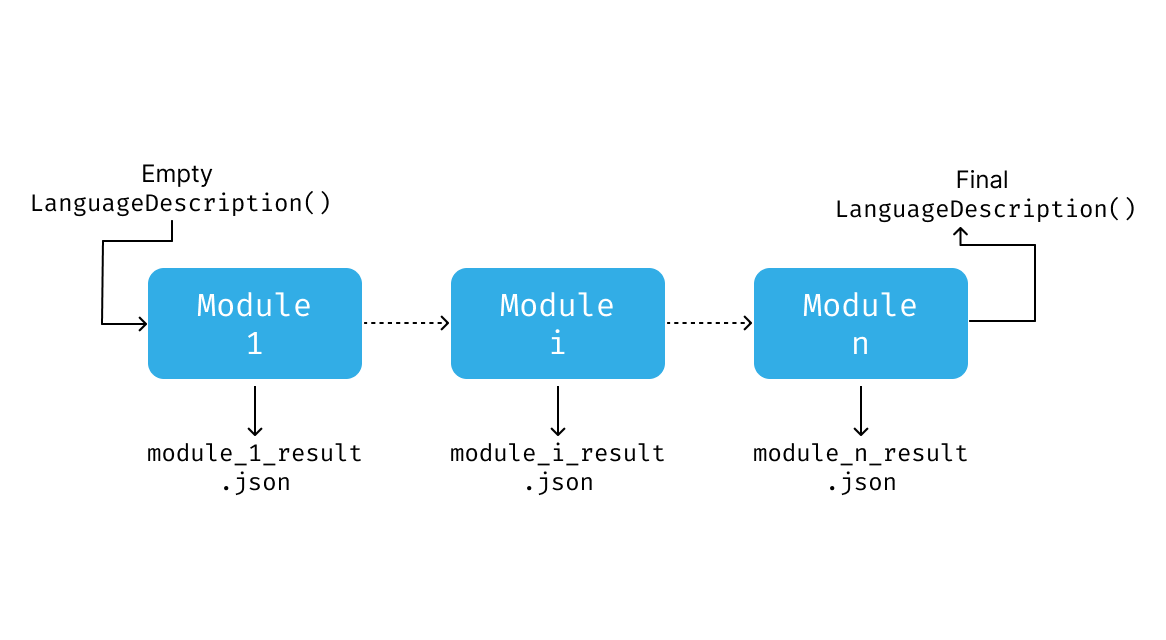
\includegraphics[width=0.8\textwidth]{figures/pipeline_structure.png}
    \caption{The pipeline structure for generating constructed languages. The modules are run in order, and each module can add or modify features of the language.}
    \label{fig:pipeline_structure}
\end{figure}

A pipeline can be setup by subclassing the \texttt{Pipeline} class, which takes care of executing the modules and saving the results. Each module of the pipeline 
is a subclass of the \texttt{Module} class, which has an \texttt{execute} method that takes a \texttt{LanguageDescription} object and other optional arguments,
and returns the modified \texttt{LanguageDescription} object and other optional results.

During the course of development, we found ourselves using more or less similar modules in most of our experiments. We have identified the following modules that are common to most
setups:

\subsection{Phonetics Modules}

The goal of a Phonetics Module is to generate the phonemic inventory of the language. The module configures the \texttt{PhonemeDataInventory} class, which
contains a list of \texttt{PhonemeData}. The phoneme segments for this class are based on PHOIBLE \cite{phoible} segments, with a \texttt{GlyphID} corresponding
to their database. For our purposes, we also implemented an \texttt{alphabet} attribute, to have a simpler representation for phonemes that are
hard to read or write. This was useful for debugging and visualization purposes.

\subsubsection{MostCommonPhonemes Module}
The \texttt{MostCommonPhonemesModule} module takes the number of consonants and vowels as arguments, and generates a phonemic inventory based on the most common
phonemes in the world languages, based on PHOIBLE \cite{phoible} data.

\subsection{Phonotactics Modules}
The goal of a Phonotactics Module is to generate the phonotactic rules of the language. The module configures the \texttt{PhonotacticData} class, which
specifies the rules for syllable structure and phonotactic constraints for word beginnings and endings.

\subsubsection{BasicPhonotacticsModule}
The \texttt{BasicPhonotacticsModule} module takes a Phonotactics string and generates a basic set of phonotactic rules. It supports defining the syllable structure
with a string of consonants and vowels, where \texttt{C} represents a consonant and \texttt{V} represents a vowel. The module also supports defining
optional consonants and vowels, by placing them in parentheses. For example, the string \texttt{(C)VC} would generate a syllable structure with an optional consonant at the beginning and
a mandatory vowel and consonant at the end.

\subsubsection{CustomPhonotacticsModule}
The \texttt{CustomPhonotacticsModule} module supports everything that the \texttt{BasicPhonotacticsModule} does, but also allows for defining
specific phonemes or set of phonemes that are allowed or not allowed in certain positions. For example, the string \texttt{C[e,o]} would generate a syllable 
structure with an consonant at the beginning and a mandatory vowel that is either \texttt{e} or \texttt{o} at the end.

\subsection{Syllable Builder Module}
The Syllable builder modules combines the phonemes generated by the Phonetics Module and the phonotactic rules generated by the Phonotactics Module to
generate all the possible syllables in the language.

\subsection{Grammar Modules}
The grammar modules generate the grammatical rules of the language. This is done by configuring the \texttt{GrammaticalFeatures} class, which contains a list of features
that inherit from either the \texttt{AbstractFeature} class or the \texttt{AbstractPOS} class. Any feature that inherits from either of these classes implements serialization and deserialization methods, 
and most importantly the \texttt{prompt\_string} method, which generates the string representation of the feature.

\subsection{BaselineAgglutinativeGrammarModule}
This is the baseline grammar module, which describes a basic agglutinative grammar. Nouns are inflected for number, case, and gender. Verbs are inflected for tense, aspect and mood.

\subsubsection{BaselineIsolatingGrammarModule}
This grammar module describes an isolating grammar, where each feature is represented by independent particles.


\subsection{Vocabulary Modules}
The goal of the Vocabulary Module is to generate the vocabulary of the language. The module configures the \texttt{VocabDictionary} class, which
holds the list of \texttt{VocabularyEntry} objects. Each \texttt{VocabularyEntry} object contains the word in the constructed language, its translation,
and its definition in english. 
A source words list is also part of each entry, to facilitate easy search for translation purposes. The class can also hold embeddings for each word, which could be also used for downstream tasks.
The vocabulary building is functionally split into two modules: Generation modules which generate the vocabulary, and Mapping modules which map the concepts with specific words. For some setups, this
is combined into a single module.

\subsubsection{FromSourceVocabularyModule}
This is a baseline generation module that takes the \texttt{n} most common words in english, and adds any missing words from the source text, and adds them to the vocabulary.

\subsubsection{ClusterTwoLevelVocabularyModule}
This is a combined vocabulary module that clusters the vocabulary into \texttt{n} clusters, based on embeddings. Each cluster is then assigned a 
root syllable, and each word in the cluster is assigned a leaf syllable. The final word is generated by concatenating the root syllable and the leaf syllable.
Agglomerative Clustering is used to cluster the vocabulary, and the number of clusters is passed as an argument to the module.

\subsubsection{ClusterAndSimplifyVocabularyModule}
This module behaves similarly to the \texttt{ClusterTwoLevelVocabularyModule}, but instead of assigning every word, each cluster is assigned a single word. 

\subsubsection{ApproximatingVocabularyModule}
This module takes a vocabulary size as argument, and generates a vocabulary of that size based on the most common words in english. Other words required for the translation
are then approximated to the closest word in the vocabulary, again based on the distance norm of the embeddings.

\subsubsection{RandomMappingModule}
This is a mapping module that randomly assigns a word to each concept in the vocabulary.

\subsection{Translation Modules}
Once the language description is generated, we use a translation module to translate some text corpora represented by \texttt{AbstractSourceText}.
The module translates the source text paragraph by paragraph, using an LLM model.

\subsection{Evaluation Modules}
Figure~\ref{fig:evaluations_structure} shows the setup for running evaluations on the generated languages. The Evaluators are a separate class 
that does not inherit from the abstract \texttt{Module} class. They inherit the \texttt{Evaluator} class, which creates an evaluations folder 
inside the results folder, to store the results of the evaluations. 

\begin{figure}
    \centering
    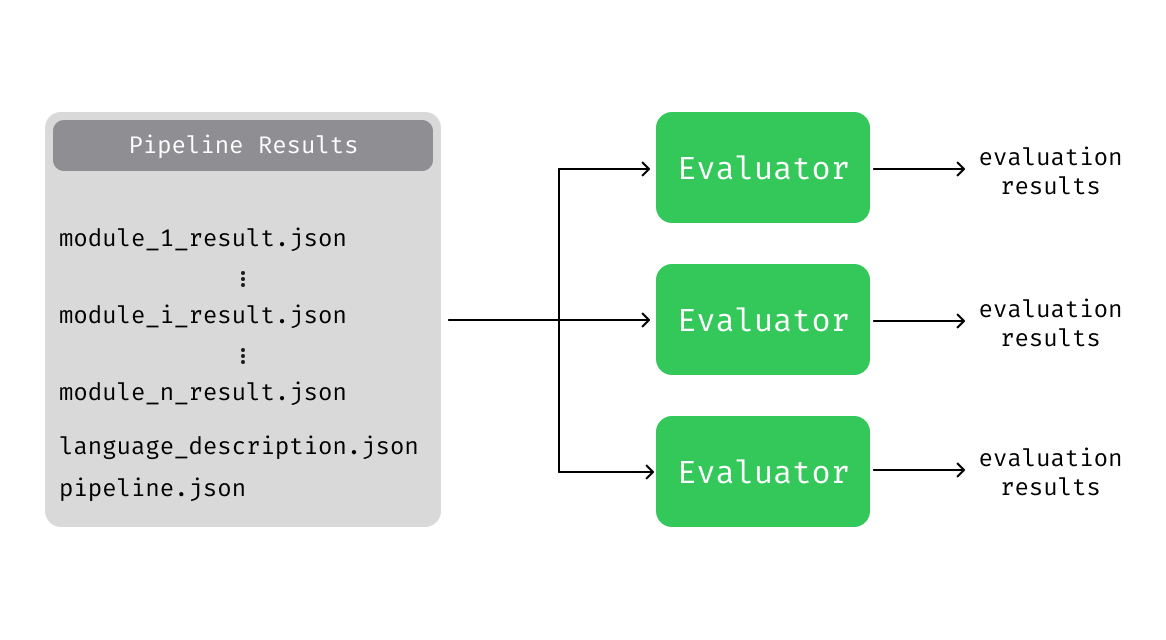
\includegraphics[width=0.8\textwidth]{figures/evaluations_structure.png}
    \caption{The setup for running evaluations. Each evaluator stores the results in a folder inside the evaluations folder.}
    \label{fig:evaluations_structure}
\end{figure}

\subsection{Pipelines}
\subsubsection{Baseline Pipeline}
 The baseline pipeline is the most straightforward pipeline, which we use to compare with different setups. Figure~\ref{fig:baseline_pipeline} shows the structure of the baseline pipeline.
 

\begin{figure}
    \centering
    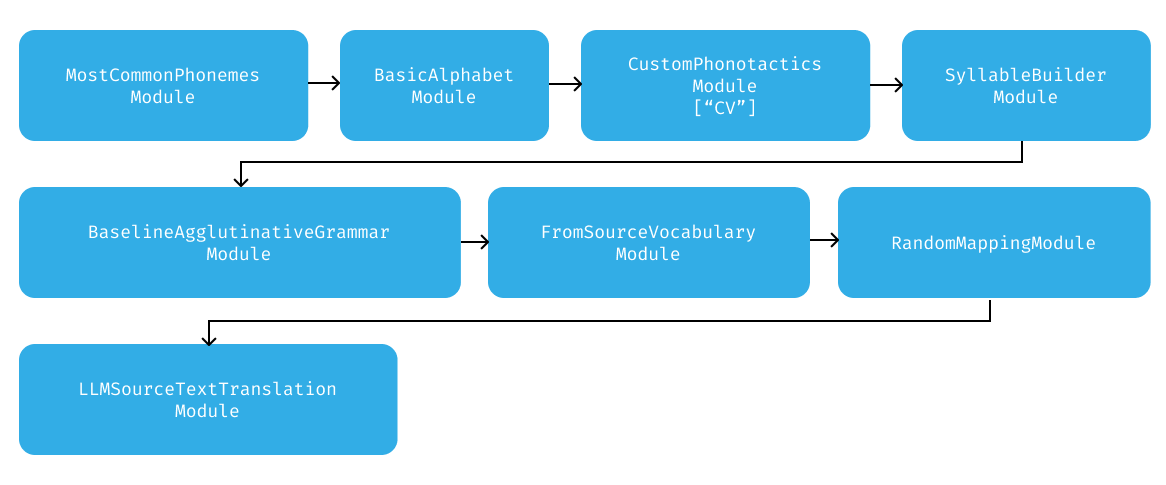
\includegraphics[width=0.8\textwidth]{figures/baseline_pipeline.png}
    \caption{The baseline pipeline for generating constructed languages.}
    \label{fig:baseline_pipeline}
\end{figure}
\subsubsection{Approximation Pipeline}
The approximation pipeline uses an approximation vocabulary module, which create a fixed vocabulary based on the most common words in english, 
and then approximates the rest of the words to the closest word in the vocabulary. Everything else is the same as the baseline pipeline.
\subsubsection{Two Level Pipeline}
The two level pipeline uses a two level vocabulary module, which clusters the vocabulary into \texttt{n} clusters, based on embeddings. Each word is bisyllabic, 
and the first syllable is the root syllable based on the cluster, and the second syllable is the leaf syllable.
\subsubsection{Cluster and Simplify Pipeline}
The cluster and simplify pipeline uses the cluster and simplify vocabulary module, which clusters the vocabulary into \texttt{n} clusters, based on embeddings.
Each cluster is assigned a single word, and the rest of the words are approximated to the closest word in the cluster.
\subsubsection{Phonotactics Pipeline}
The phonotactics pipeline uses the \texttt{CustomPhonotacticsModule}. As compared to the baseline pipeline which uses the \texttt{CV} syllable structure,
This pipeline uses custom phonotactic rules. The rest of the pipeline is the same as the baseline pipeline.

\subsection{LLMs and Embedders}
We used both Local and Remote LLMs for our experiments. The use of Local LLMs is facilitated by the \texttt{LocalLLM} class, which is a wrapper 
to access local LLMs via the Ollama Library. The Remote LLMs are accessed via the \texttt{RemoteLLM} class, which supports two providers: OpenAI and Groq.
The primary models used for the experiments were \textit{deepseek-r1:14b} and OpenAI's \textit{gpt-4o}.  

For the embedding models, we primarily used the \textit{all-MiniLM-L6-v2} model from HuggingFace.

\subsection{Clustering}
We used the \textit{AgglomerativeClustering} class from the \textit{sklearn} library for clustering the vocabulary, which we noticed gave the best 
results heuristically.
